\begin{figure}
  \begin{subfigure}{0.3225806451612903\textwidth}
  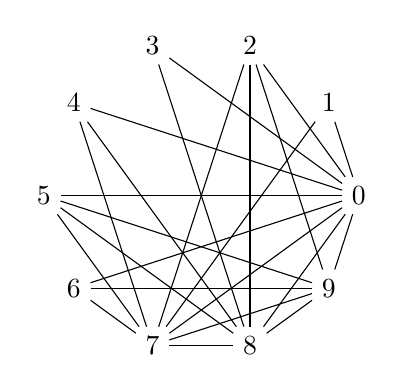
\begin{tikzpicture}
      \draw
        (0.0:2) node (0){0}
        (36.0:2) node (1){1}
        (72.0:2) node (2){2}
        (108.0:2) node (3){3}
        (144.0:2) node (4){4}
        (180.0:2) node (5){5}
        (216.0:2) node (6){6}
        (252.0:2) node (7){7}
        (288.0:2) node (8){8}
        (324.0:2) node (9){9};
      \begin{scope}[-]
        \draw (0) to (1);
        \draw (0) to (2);
        \draw (0) to (3);
        \draw (0) to (4);
        \draw (0) to (5);
        \draw (0) to (6);
        \draw (0) to (7);
        \draw (0) to (8);
        \draw (0) to (9);
        \draw (1) to (7);
        \draw (2) to (7);
        \draw (2) to (8);
        \draw (2) to (9);
        \draw (3) to (8);
        \draw (4) to (7);
        \draw (4) to (8);
        \draw (5) to (7);
        \draw (5) to (8);
        \draw (5) to (9);
        \draw (6) to (7);
        \draw (6) to (9);
        \draw (7) to (8);
        \draw (7) to (9);
        \draw (8) to (9);
      \end{scope}
    \end{tikzpicture}
    \caption{Small-world topology}\label{small-world}
  \end{subfigure}
  \begin{subfigure}{0.3225806451612903\textwidth}
  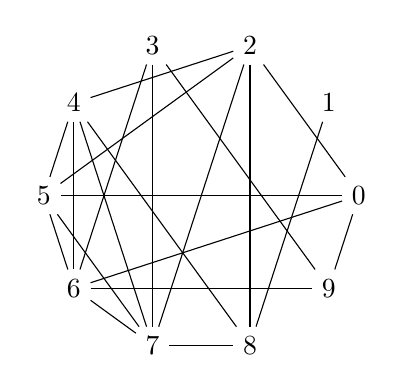
\begin{tikzpicture}
      \draw
        (0.0:2) node (0){0}
        (36.0:2) node (1){1}
        (72.0:2) node (2){2}
        (108.0:2) node (3){3}
        (144.0:2) node (4){4}
        (180.0:2) node (5){5}
        (216.0:2) node (6){6}
        (252.0:2) node (7){7}
        (288.0:2) node (8){8}
        (324.0:2) node (9){9};
      \begin{scope}[-]
        \draw (0) to (2);
        \draw (0) to (5);
        \draw (0) to (6);
        \draw (0) to (9);
        \draw (1) to (8);
        \draw (2) to (4);
        \draw (2) to (5);
        \draw (2) to (7);
        \draw (2) to (8);
        \draw (3) to (6);
        \draw (3) to (7);
        \draw (3) to (9);
        \draw (4) to (5);
        \draw (4) to (6);
        \draw (4) to (7);
        \draw (4) to (8);
        \draw (5) to (6);
        \draw (5) to (7);
        \draw (6) to (7);
        \draw (6) to (9);
        \draw (7) to (8);
      \end{scope}
    \end{tikzpicture}
    \caption{Random topology}\label{random}
  \end{subfigure}
  \begin{subfigure}{0.3225806451612903\textwidth}
  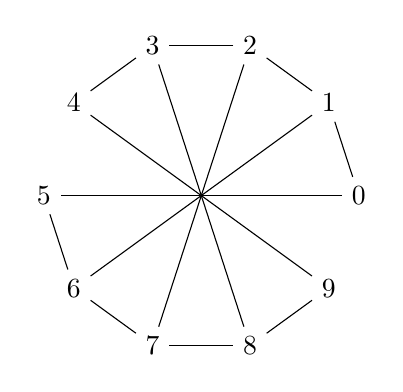
\begin{tikzpicture}
      \draw
        (0.0:2) node (0){0}
        (36.0:2) node (1){1}
        (72.0:2) node (2){2}
        (108.0:2) node (3){3}
        (144.0:2) node (4){4}
        (180.0:2) node (5){5}
        (216.0:2) node (6){6}
        (252.0:2) node (7){7}
        (288.0:2) node (8){8}
        (324.0:2) node (9){9};
      \begin{scope}[-]
        \draw (0) to (1);
        \draw (0) to (5);
        \draw (1) to (2);
        \draw (1) to (6);
        \draw (2) to (3);
        \draw (2) to (7);
        \draw (3) to (4);
        \draw (3) to (8);
        \draw (4) to (9);
        \draw (5) to (6);
        \draw (6) to (7);
        \draw (7) to (8);
        \draw (8) to (9);
      \end{scope}
    \end{tikzpicture}
    \caption{Ladder topology}\label{ladder}
  \end{subfigure}
  \begin{subfigure}{0.3225806451612903\textwidth}
  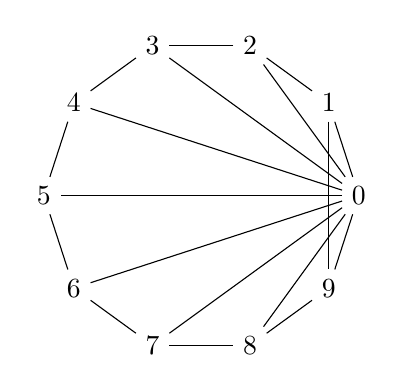
\begin{tikzpicture}
      \draw
        (0.0:2) node (0){0}
        (36.0:2) node (1){1}
        (72.0:2) node (2){2}
        (108.0:2) node (3){3}
        (144.0:2) node (4){4}
        (180.0:2) node (5){5}
        (216.0:2) node (6){6}
        (252.0:2) node (7){7}
        (288.0:2) node (8){8}
        (324.0:2) node (9){9};
      \begin{scope}[-]
        \draw (0) to (1);
        \draw (0) to (2);
        \draw (0) to (3);
        \draw (0) to (4);
        \draw (0) to (5);
        \draw (0) to (6);
        \draw (0) to (7);
        \draw (0) to (8);
        \draw (0) to (9);
        \draw (1) to (2);
        \draw (1) to (9);
        \draw (2) to (3);
        \draw (3) to (4);
        \draw (4) to (5);
        \draw (5) to (6);
        \draw (6) to (7);
        \draw (7) to (8);
        \draw (8) to (9);
      \end{scope}
    \end{tikzpicture}
    \caption{Wheel topology}\label{wheel}
  \end{subfigure}
  \begin{subfigure}{0.3225806451612903\textwidth}
  \begin{tikzpicture}
      \draw
        (0.0:2) node (0){0}
        (36.0:2) node (1){1}
        (72.0:2) node (2){2}
        (108.0:2) node (3){3}
        (144.0:2) node (4){4}
        (180.0:2) node (5){5}
        (216.0:2) node (6){6}
        (252.0:2) node (7){7}
        (288.0:2) node (8){8}
        (324.0:2) node (9){9};
      \begin{scope}[-]
        \draw (0) to (1);
        \draw (1) to (2);
        \draw (2) to (3);
        \draw (3) to (4);
        \draw (4) to (5);
        \draw (5) to (6);
        \draw (6) to (7);
        \draw (7) to (8);
        \draw (8) to (9);
      \end{scope}
    \end{tikzpicture}
    \caption{Pipeline topology}\label{pipeline}
  \end{subfigure}
  \begin{subfigure}{0.3225806451612903\textwidth}
  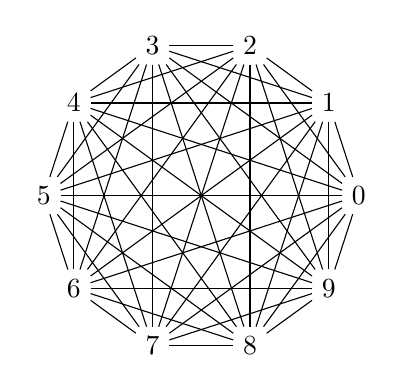
\begin{tikzpicture}
      \draw
        (0.0:2) node (0){0}
        (36.0:2) node (1){1}
        (72.0:2) node (2){2}
        (108.0:2) node (3){3}
        (144.0:2) node (4){4}
        (180.0:2) node (5){5}
        (216.0:2) node (6){6}
        (252.0:2) node (7){7}
        (288.0:2) node (8){8}
        (324.0:2) node (9){9};
      \begin{scope}[-]
        \draw (0) to (1);
        \draw (0) to (2);
        \draw (0) to (3);
        \draw (0) to (4);
        \draw (0) to (5);
        \draw (0) to (6);
        \draw (0) to (7);
        \draw (0) to (8);
        \draw (0) to (9);
        \draw (1) to (2);
        \draw (1) to (3);
        \draw (1) to (4);
        \draw (1) to (5);
        \draw (1) to (6);
        \draw (1) to (7);
        \draw (1) to (8);
        \draw (1) to (9);
        \draw (2) to (3);
        \draw (2) to (4);
        \draw (2) to (5);
        \draw (2) to (6);
        \draw (2) to (7);
        \draw (2) to (8);
        \draw (2) to (9);
        \draw (3) to (4);
        \draw (3) to (5);
        \draw (3) to (6);
        \draw (3) to (7);
        \draw (3) to (8);
        \draw (3) to (9);
        \draw (4) to (5);
        \draw (4) to (6);
        \draw (4) to (7);
        \draw (4) to (8);
        \draw (4) to (9);
        \draw (5) to (6);
        \draw (5) to (7);
        \draw (5) to (8);
        \draw (5) to (9);
        \draw (6) to (7);
        \draw (6) to (8);
        \draw (6) to (9);
        \draw (7) to (8);
        \draw (7) to (9);
        \draw (8) to (9);
      \end{scope}
    \end{tikzpicture}
    \caption{Complete topology}\label{complete}
  \end{subfigure}
  \caption{Examples of topologies.}\label{fig:topologies}
\end{figure}